%\subsection{Schema generale: addestramento degli algoritmi di predizione con applicativo esterno con estensioni}
%\begin{figure}[H]
%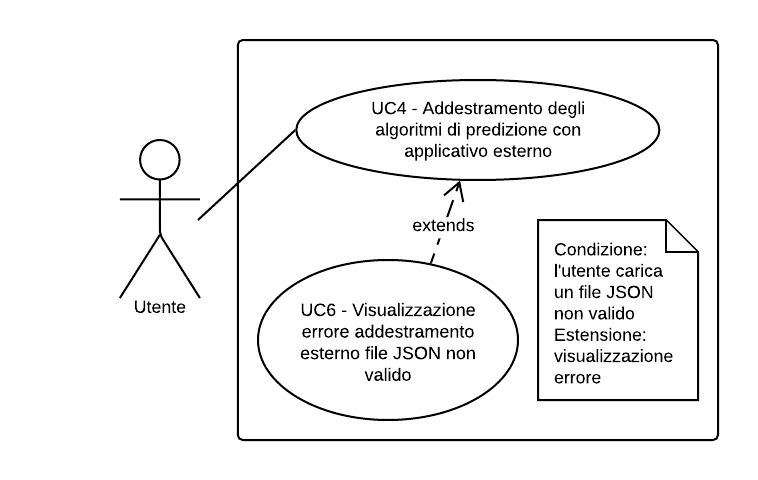
\includegraphics{img/UC4 - Schema generale.png}
%\caption{Schema generale: addestramento degli algoritmi di predizione con applicativo esterno con estensioni}
%\end{figure}
\subsection{UC4 - Addestramento degli algoritmi di predizione con applicativo esterno}
\begin{itemize}
    \item \textbf{Codice identificativo}: UC4;
    \item \textbf{Titolo}: addestramento degli algoritmi di predizione con applicativo esterno;
    \item \textbf{Attori primari}: utente;
    \item \textbf{Descrizione}: attività di addestramento degli algoritmi di predizione eseguita nell'applicativo esterno a Grafana\glosp utilizzando dei dati inseriti da un utente;
    \item \textbf{Precondizioni}: l'utente è autenticato nel sistema software Grafana\glo;
    \item \textbf{Postcondizioni}: l'utente ha completato l'addestramento degli algoritmi di predizione;
    \item \textbf{Scenario principale}: 
        \begin{enumerate}
            \item inserimento del file in formato CSV contenente i dati per l'addestramento (UC4.1);
            \item visualizzazione grafico dei dati per l'addestramento (UC4.6);
            \item inserimento del file in formato JSON contenente i dati di una configurazione precedente (UC4.7);
            \item inserimento delle note per l'utente (UC4.8);
            \item selezione del modello di predizione su cui eseguire l'addestramento (UC4.2);
            \item avvio dell'addestramento (UC4.3);
            \item ricezione del file JSON contenente i predittori (UC4.5);
            \item visualizzazione del messaggio di conferma della conclusione dell'addestramento (UC4.9). 
        \end{enumerate}
    \item \textbf{Scenari alternativi}:
    \begin{enumerate}
    	\item arresto dell'addestramento (UC4.4).
    \end{enumerate}
    \item \textbf{Estensioni}:
    \begin{enumerate}
    	\item se il caricamento del file CSV non è avvenuto con successo viene visualizzato un messaggio di errore (UC18);
    	\item se il caricamento del file JSON non è avvenuto con successo viene visualizzato un messaggio di errore (UC6).
    \end{enumerate}
\end{itemize}

\subsubsection{UC4.1 - Inserimento del file in formato CSV contenente i dati per l'addestramento}
\begin{itemize}
    \item \textbf{Codice identificativo}: UC4.1;
    \item \textbf{Titolo}: inserimento del file in formato CSV contenente i dati per l'addestramento;
    \item \textbf{Attori primari}: utente;
    \item \textbf{Descrizione}: l'utente inserisce un file in formato CSV contenente i dati per l'addestramento nell'applicazione esterna;
    \item \textbf{Precondizioni}: l'utente è autenticato nel sistema software Grafana\glo;
    \item \textbf{Postcondizioni}: l'utente ha inserito correttamente il file in formato CSV contenente i dati per l'addestramento;
    \item \textbf{Scenario principale}: l'utente inserisce il file in formato CSV contenente i dati per l'addestramento.
\end{itemize}
\subsubsection{UC4.6 - Visualizzazione grafico dei dati per l'addestramento}
\begin{itemize}
	\item \textbf{Codice identificativo}: UC4.6;
	\item \textbf{Titolo}: visualizzazione grafico dei dati per l'addestramento;
	\item \textbf{Attori primari}: utente;
	\item \textbf{Descrizione}: l'utente visualizza il grafico a dispersione rappresentante i dati che ha inserito per l'addestramento;
	\item \textbf{Precondizioni}: il file CSV contenente i dati per l'addestramento è stato inserito correttamente nell'applicazione esterna;
	\item \textbf{Postcondizioni}: l'utente ha visualizzato il grafico a dispersione rappresentante i dati che ha inserito;
	\item \textbf{Scenario principale}: l'utente visualizza il grafico a dispersione rappresentante i dati che ha inserito.
\end{itemize}
\subsubsection{UC4.7 - Inserimento del file in formato JSON contenente una configurazione precedente}
\begin{itemize}
	\item \textbf{Codice identificativo}: UC4.7;
	\item \textbf{Titolo}: inserimento del file in formato JSON contenente una configurazione precedente;
	\item \textbf{Attori primari}: utente;
	\item \textbf{Descrizione}: l'utente inserisce nell'applicazione esterna un file in formato JSON che contiene i dati di una configurazione per addestrare nuovamente l'algoritmo di predizione partendo con una configurazione precedente;
	\item \textbf{Precondizioni}: l'utente è autenticato nel sistema software Grafana\glo;
	\item \textbf{Postcondizioni}: il file in formato JSON contenente una configurazione precedente è stato inserito correttamente;
	\item \textbf{Scenario principale}: l'utente inserisce il file in formato JSON contenente una configurazione precedente.
\end{itemize}
\subsubsection{UC4.8 - Inserimento delle note per l'utente}
\begin{itemize}
	\item \textbf{Codice identificativo}: UC4.8;
	\item \textbf{Titolo}: inserimento delle note per l'utente;
	\item \textbf{Attori primari}: utente;
	\item \textbf{Descrizione}: l'utente inserisce le note che compariranno nel file JSON risultante dall'addestramento dell'algoritmo;
	\item \textbf{Precondizioni}: il file CSV contenente i dati per l'addestramento è stato inserito correttamente nell'applicazione esterna;
	\item \textbf{Postcondizioni}: l'utente ha inserito correttamente le note che compariranno nel file JSON risultante dall'addestramento dell'algoritmo;
	\item \textbf{Scenario principale}: l'utente inserisce le note che compariranno nel file JSON risultante dall'addestramento dell'algoritmo.
\end{itemize}
\subsubsection{UC4.2 - Selezione del modello di predizione su cui eseguire l'addestramento}
\begin{itemize}
    \item \textbf{Codice identificativo}: UC4.2;
    \item \textbf{Titolo}: selezione del modello di predizione su cui eseguire l'addestramento;
    \item \textbf{Attori primari}: utente;
    \item \textbf{Descrizione}: l'utente seleziona il modello di predizione da applicare durante l'addestramento;
    \item \textbf{Precondizioni}: il file CSV contenente i dati per l'addestramento è stato inserito correttamente nell'applicazione esterna;
    \item \textbf{Postcondizioni}: il modello di predizione è stato selezionato correttamente;
    \item \textbf{Scenario principale}: l'utente seleziona un modello di predizione su cui eseguire l'addestramento tra SVM\glosp e RL\glo;
    \item \textbf{Specializzazione}:
    \begin{itemize}
    	\item selezione del modello di predizione SVM\glosp (UC4.10);
    	\item selezione del modello di predizione RL\glosp (UC4.11).
    \end{itemize}   
\end{itemize}
\subsubsection{UC4.10 - Selezione del modello di predizione SVM}
\begin{itemize}
	\item \textbf{Codice identificativo}: UC4.10;
	\item \textbf{Titolo}: selezione del modello di predizione SVM\glo;
	\item \textbf{Attori primari}: utente;
	\item \textbf{Descrizione}: l'utente seleziona il modello di predizione SVM\glosp da applicare durante l'addestramento nell'applicazione esterna;
	\item \textbf{Precondizioni}: il file CSV contenente i dati per l'addestramento è stato inserito correttamente nell'applicazione esterna;
	\item \textbf{Postcondizioni}: l'utente ha selezionato SVM\glosp come modello di predizione da applicare;
	\item \textbf{Scenario principale}: l'utente seleziona il modello di predizione SVM\glosp su cui eseguire l'addestramento.
\end{itemize}
\subsubsection{UC4.11 - Selezione del modello di predizione RL}
\begin{itemize}
	\item \textbf{Codice identificativo}: UC4.11;
	\item \textbf{Titolo}: selezione del modello di predizione RL\glo;
	\item \textbf{Attori primari}: utente;
	\item \textbf{Descrizione}: l'utente seleziona il modello di predizione RL\glosp da applicare durante l'addestramento nell'applicazione esterna;
	\item \textbf{Precondizioni}: il file CSV contenente i dati per l'addestramento è stato inserito correttamente nell'applicazione esterna;
	\item \textbf{Postcondizioni}: l'utente ha selezionato RL\glosp come modello di predizione da applicare;
	\item \textbf{Scenario principale}: l'utente seleziona il modello di predizione RL\glosp su cui eseguire l'addestramento.
\end{itemize}
\subsubsection{UC4.12 - Selezione del modello di predizione reti neurali}
\begin{itemize}
	\item \textbf{Codice identificativo}: UC4.12;
	\item \textbf{Titolo}: selezione del modello di predizione reti neurali;
	\item \textbf{Attori primari}: utente;
	\item \textbf{Attori secondari}: Grafana\glo;
	\item \textbf{Descrizione}: l'utente seleziona reti neurali come modello di predizione da applicare durante l'addestramento;
	\item \textbf{Precondizioni}: l'utente è autenticato nel sistema software Grafana\glosp e il file CSV contenente i dati per l'addestramento è stato inserito correttamente;
	\item \textbf{Postcondizioni}: l'utente ha selezionato reti neurali come modello di predizione da applicare;
	\item \textbf{Scenario principale}: l'utente seleziona il modello di predizione reti neurali su cui eseguire l'addestramento.
\end{itemize}
\subsubsection{UC4.13 - Selezione del modello di predizione regressioni esponenziali}
\begin{itemize}
	\item \textbf{Codice identificativo}: UC4.13;
	\item \textbf{Titolo}: selezione del modello di predizione regressioni esponenziali;
	\item \textbf{Attori primari}: utente;
	\item \textbf{Attori secondari}: Grafana\glo;
	\item \textbf{Descrizione}: l'utente seleziona regressioni esponenziali come modello di predizione da applicare durante l'addestramento;
	\item \textbf{Precondizioni}: l'utente è autenticato nel sistema software Grafana\glosp e il file CSV contenente i dati per l'addestramento è stato inserito correttamente;
	\item \textbf{Postcondizioni}: l'utente ha selezionato regressioni esponenziali come modello di predizione da applicare;
	\item \textbf{Scenario principale}: l'utente seleziona il modello di predizione regressioni esponenziali su cui eseguire l'addestramento.
\end{itemize}
\subsubsection{UC4.14 - Selezione del modello di predizione regressioni logaritmiche}
\begin{itemize}
	\item \textbf{Codice identificativo}: UC4.14;
	\item \textbf{Titolo}: selezione del modello di predizione regressioni logaritmiche;
	\item \textbf{Attori primari}: utente;
	\item \textbf{Attori secondari}: Grafana\glo;
	\item \textbf{Descrizione}: l'utente seleziona regressioni logaritmiche come modello di predizione da applicare durante l'addestramento;
	\item \textbf{Precondizioni}: l'utente è autenticato nel sistema software Grafana\glosp e il file CSV contenente i dati per l'addestramento è stato inserito correttamente;
	\item \textbf{Postcondizioni}: l'utente ha selezionato regressioni logaritmiche come modello di predizione da applicare;
	\item \textbf{Scenario principale}: l'utente seleziona il modello di predizione regressioni logaritmiche su cui eseguire l'addestramento.
\end{itemize}
\subsubsection{UC4.15 - Selezione del modello di predizione SVM adattata alla Regressione}
\begin{itemize}
	\item \textbf{Codice identificativo}: UC4.15;
	\item \textbf{Titolo}: selezione del modello di predizione SVM adattata alla Regressione;
	\item \textbf{Attori primari}: utente;
	\item \textbf{Attori secondari}: Grafana\glo;
	\item \textbf{Descrizione}: l'utente seleziona SVM adattata alla Regressione come modello di predizione da applicare durante l'addestramento;
	\item \textbf{Precondizioni}: l'utente è autenticato nel sistema software Grafana\glosp e il file CSV contenente i dati per l'addestramento è stato inserito correttamente;
	\item \textbf{Postcondizioni}: l'utente ha selezionato SVM adattata alla Regressione come modello di predizione da applicare;
	\item \textbf{Scenario principale}: l'utente seleziona il modello di predizione SVM adattata alla Regressione su cui eseguire l'addestramento.
\end{itemize}
\subsubsection{UC4.3 - Avvio dell'addestramento}
\begin{itemize}
    \item \textbf{Codice identificativo}: UC4.3;
    \item \textbf{Titolo}: avvio dell'addestramento;
    \item \textbf{Attori primari}: utente;
    \item \textbf{Descrizione}: l'utente avvia l'addestramento dell'algoritmo di predizione;
    \item \textbf{Precondizioni}: il file CSV è stato inserito correttamente e il modello di predizione è stato selezionato;
    \item \textbf{Postcondizioni}: l'addestramento è stato avviato con successo;
    \item \textbf{Scenario principale}: l'utente avvia l'addestramento.
\end{itemize}

\subsubsection{UC4.4 - Arresto dell'addestramento}
\begin{itemize}
	\item \textbf{Codice identificativo}: UC4.4;
	\item \textbf{Titolo}: arresto dell'addestramento;
	\item \textbf{Attori primari}: utente;
	\item \textbf{Descrizione}: l'utente arresta l'addestramento prima della sua normale conclusione;
	\item \textbf{Precondizioni}: l'addestramento è stato avviato con successo;
	\item \textbf{Postcondizioni}: l'addestramento è stato arrestato con successo;
	\item \textbf{Scenario principale}: l'utente arresta forzatamente l'addestramento.
\end{itemize}

\subsubsection{UC4.9 - Visualizzazione del messaggio di conferma della conclusione dell'addestramento}
\begin{itemize}
	\item \textbf{Codice identificativo}: UC4.9;
	\item \textbf{Titolo}: visualizzazione del messaggio di conferma della conclusione dell'addestramento;
	\item \textbf{Attori primari}: utente;
	\item \textbf{Descrizione}: l'utente visualizza un messaggio di conferma che l'addestramento è stato concluso ed eseguito correttamente;
	\item \textbf{Precondizioni}: l'addestramento è stato avviato con successo;
	\item \textbf{Postcondizioni}: l'utente ha visualizzato un messaggio di conferma che l'addestramento è stato concluso ed eseguito correttamente;
	\item \textbf{Scenario principale}: l'utente visualizza un messaggio di conferma che l'addestramento è stato concluso ed eseguito correttamente.
\end{itemize}

\subsubsection{UC4.5 - Ricezione del file JSON contente i predittori}
\begin{itemize}
    \item \textbf{Codice identificativo}: UC4.5;
    \item \textbf{Titolo}: ricezione del file JSON contenente i predittori;
    \item \textbf{Attori primari}: utente;
    \item \textbf{Descrizione}: l'applicazione restituisce un file JSON, risultato dal completamento dell'addestramento dei dati, contenente i predittori per eseguire la predizione;
    \item \textbf{Precondizioni}: l'applicazione esterna ha concluso l'addestramento con successo secondo il suo normale flusso di esecuzione;
    \item \textbf{Postcondizioni}: l'utente ha ricevuto il file JSON, risultato dall'addestramento, contenente i predittori per eseguire la predizione;
    \item \textbf{Scenario principale}: l'utente riceve il file JSON, risultato dall'addestramento, contenente i predittori per eseguire la predizione.
\end{itemize}